\documentclass[t, notes, xcolor=table]{beamer}

\usepackage{wrapfig}
\usepackage{float}
% For tabs in verbatim
\usepackage{fancyvrb}

% Adjust position of the image
\usepackage[export]{adjustbox}

% set fonts
\usefonttheme{professionalfonts} % using non standard fonts for beamer
\usepackage{txfonts,mathptmx}

% set indend spacing for first and second level indentation
\setlength{\leftmargini}{0.5cm}
\setlength{\leftmarginii}{0.5cm}
\setlength{\leftmarginiii}{0.5cm}

% Set circles for bullets 
\setbeamertemplate{itemize items}[circle]

% colors
\usepackage{xcolor}

% multiple columns
\usepackage{multicol}

% todo lists
\usepackage{pifont}
\usepackage{amssymb}

% increase space between text and frame name
\addtobeamertemplate{frametitle}{}{\vspace{0.5em}}

%Information to be included in the title page:
\title{Understanding the Simulation Cycle}
\author{Nikola Petrovic}
\institute{University of Belgrade, School of Electrical Engineering}
\date{2022}



\begin{document}

\frame{\titlepage}

%%%%%%%%%%%%%%%%%%%%%%%%%%%%%%%%%%%%%%%%%%%%%%%%%%%%%%%%%%%%
\begin{frame}
\frametitle{Module Objective}

In this module we will produce high quality code that is less subject to non-determinism and race conditions.
\newline

\textbf{Topics:}
\begin{itemize}
\item Procedural blocks and event control review
\item Blocking procedural assignment review
\item Making non-blocking procedural assignments
\item Non-blocking assignments and the simulation cycle
\item Synchronizing procedures
\begin{itemize}
	\item With event controls
	\item With level-sensitive event controls
	\item With procedural delay controls
\end{itemize}
\end{itemize}

\end{frame}
\note{
\scriptsize{
Out objective is to produce high-quality code less prone to indeterminacy and race conditions. To do that, we need to understand something about how the simulator executes processes and their statements. Some terminology definitions are as below:
\begin{itemize}
\item \textbf{Simulation time}: Time value maintained by the simulator to model the actual time it would take for the circuit being simulated
\item \textbf{Process}: Verilog code to evaluate, e.q., \textit{always} and \textit{initial} blocks and continuous assignments
\item \textbf{Evaluation Event}: Evaluation of a process
\item \textbf{Update Event}: Change in value of a net or variable
\item \textbf{Event Queue}: Queue of events, ordered by simulation time
\item \textbf{Scheduling an Event}: Putting an event onto the event queue
\item \textbf{Simulation Cycle}: Processing all active events in the event queue
\end{itemize}

}
}

%%%%%%%%%%%%%%%%%%%%%%%%%%%%%%%%%%%%%%%%%%%%%%%%%%%%%%%%%%%%
\begin{frame}
\frametitle{Procedural Blocks and Event Control Review}

\tiny{
\begin{multicols}{2}
An \textcolor{purple}{always} construct is a procedural block that loops continuously throughout the simulation.
\newline

An \textcolor{purple}{initial} construct is a procedural block that executes once.
\newline

The \textbf{@} token introduces an event control, blocking further execution for either:
\begin{itemize}
\item A single event identifier
\item An event expression
\begin{itemize}
	\tiny{
	\item Can create an event list with \textbf{or} and comma "\textbf{,}" operators
	\item Can qualify an expression term with \textbf{posedge} or \textbf{negedge}	
	}
\end{itemize}
\end{itemize}
Can give a block a name.
\newline

Combinational logic can use the blocking assignment "\textbf{=}" operator.
\newline

Sequential logic must use the non-blocking assignment "\textbf{\textless =}" operator.
\newline

Multiple procedures execute "concurrently".
\vfill
\columnbreak
\begin{figure}
    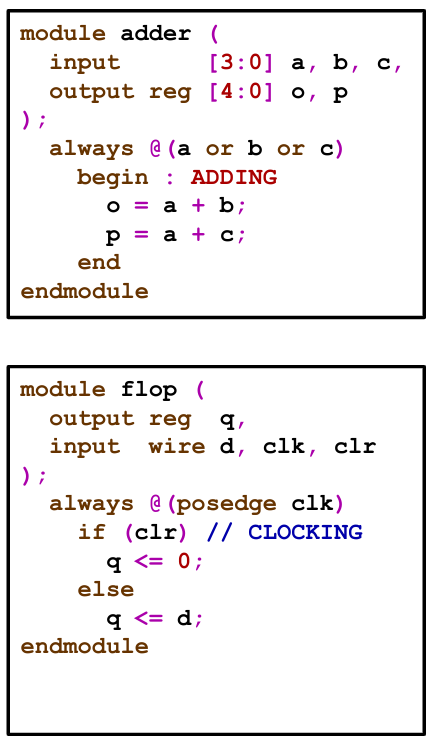
\includegraphics[width=0.45\textwidth]{img/09_proc_event_review.png}
\end{figure}
\end{multicols}

}
\end{frame}
\note{
\tiny{
An \textbf{always} construct is a procedural block that loops continuously throughout the simulation.
\newline

An \textbf{initial} construct is a procedural block that executes once.
\newline

The \textbf{@} token introduces an event control, which blocks further execution until an event occurs. The event control can utilize a single event identifier or it can utilize an event expression that may be a list of event expressions separated by the \textbf{or} token or separated by commas with terms that can be qualified with \textit{posedge} or \textit{negedge} qualifiers.
\newline

We can name a sequential block by appending a colon and identifier to the \textit{begin} keyword. A named block creates another level of scope that can declare its own variables. Of course we can always just make a pertinent comment about the statement's purpose.
\newline

A procedural block that represents combinational logic can use the blocking assignment (\textbf{=}) operator.
\newline

A procedural block that represents sequential logic must use the non-blocking assignment (\textbf{\textless =}) operator.
\newline

Multiple procedural blocks execute in a manner that appears \textit{concurrent} to the user. Multiple procedural blocks scheduled to execute in the same simulation cycle can execute in any order.

}
}


%%%%%%%%%%%%%%%%%%%%%%%%%%%%%%%%%%%%%%%%%%%%%%%%%%%%%%%%%%%%
\begin{frame}
\frametitle{Blocking Procedural Assignment Review}
\scriptsize{
\begin{multicols}{2}
Blocking assignment "\textbf{=}" operator.
\newline

Blocks execution of subsequent statements until assignment completes:
\begin{itemize}
	\item By default immediately
	\item Later slides show how to delay	
\end{itemize}
\

Almost all examples so far have used blocking assignments.
\newline

This cause problems with some code structures.

\vfill
\columnbreak
\begin{figure}
    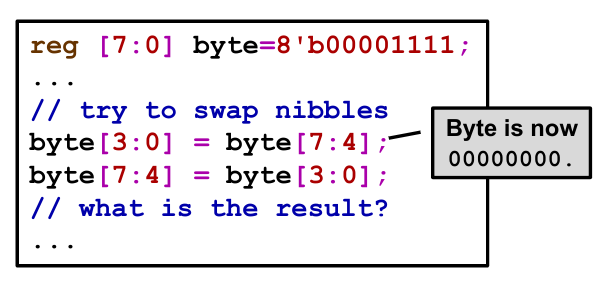
\includegraphics[width=0.45\textwidth]{img/09_block_review.png}
\end{figure}
\end{multicols}
}
\end{frame}
\note{
\scriptsize{
The procedural assignments we have seen so far are blocking assignments. They are called blocking because they block the execution of the next statement until they complete. This ensures that future statements can use the new value of the updated variable. We will often see it written that these assignments are \textit{immediate}, but that is not necessarily true, as we will see later how to deliberately delay them.
\newline

This illustration attempts to use blocking assignments to swap the upper and lower halves of a byte. It first assigns the upper half to the lower half and then assigns the lower half to the upper half. This does not have the desired effect, as the simulator completes the first assignment before it starts the second assignment. At the end of the first assignment, both halves have the same value.
\newline

We can work around such affects by utilizing a temporary variable, but an even better solution performs both assignments in a way that appears concurrent.

}
}


%%%%%%%%%%%%%%%%%%%%%%%%%%%%%%%%%%%%%%%%%%%%%%%%%%%%%%%%%%%%
\begin{frame}
\frametitle{Non-blocking Procedural Assignment Review}
\scriptsize{
\begin{multicols}{2}
Non-blocking assignment "\textcolor{purple}{\textless =}" operator:
\begin{itemize}
\item RHS expression values is \textit{calculated}
\item LHS variable update is \textit{scheduled}
\end{itemize}
\vfill
\columnbreak
\begin{figure}
    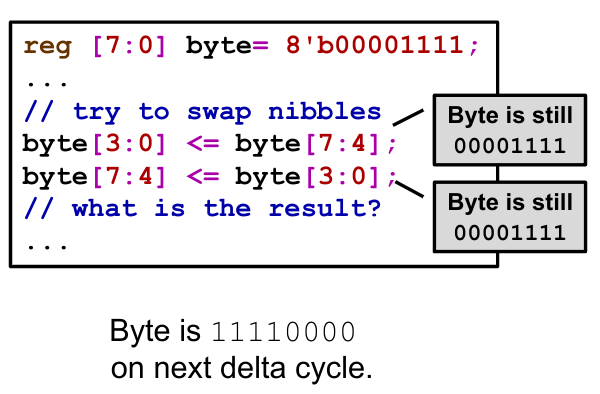
\includegraphics[width=0.45\textwidth]{img/09_nonblock_review.png}
\end{figure}
\end{multicols}
}
\end{frame}
\note{
\scriptsize{
We can alternatively make non-blocking assignments. They are called non-blocking assignments because their completion is scheduled and they do not block the execution of the next statement. The simulator instead calculates and retains the new value, but schedules the actual variable update for a point in the simulation where all currently triggered blocks have executed up to the point where they are all blocked. This ensures that any other triggered block that reads the variable reads the old value and not the new one.
\newline

Non-blocking assignments use the same token as the less-than-or-equal-to (\textless =) operator. it may be helpful to us to remember that non-blocking word is longer than the blocking word and that the non-blocking operator is longer than the blocking operator.
\newline

This illustration uses the non-blocking assignments to swap the upper and lower halves of the byte. It first assigns the upper half to the lower half and then it assigns the lower half to the upper half. This \textbf{does} have the desired affect, as the simulator evaluates the first assignment after completing the second assignment. The simulator does not update the value of the variable until the procedural block next blocks at the event control.

}
}



%%%%%%%%%%%%%%%%%%%%%%%%%%%%%%%%%%%%%%%%%%%%%%%%%%%%%%%%%%%%
\begin{frame}
\frametitle{Simplified Stratified Event Queue}
\begin{figure}
    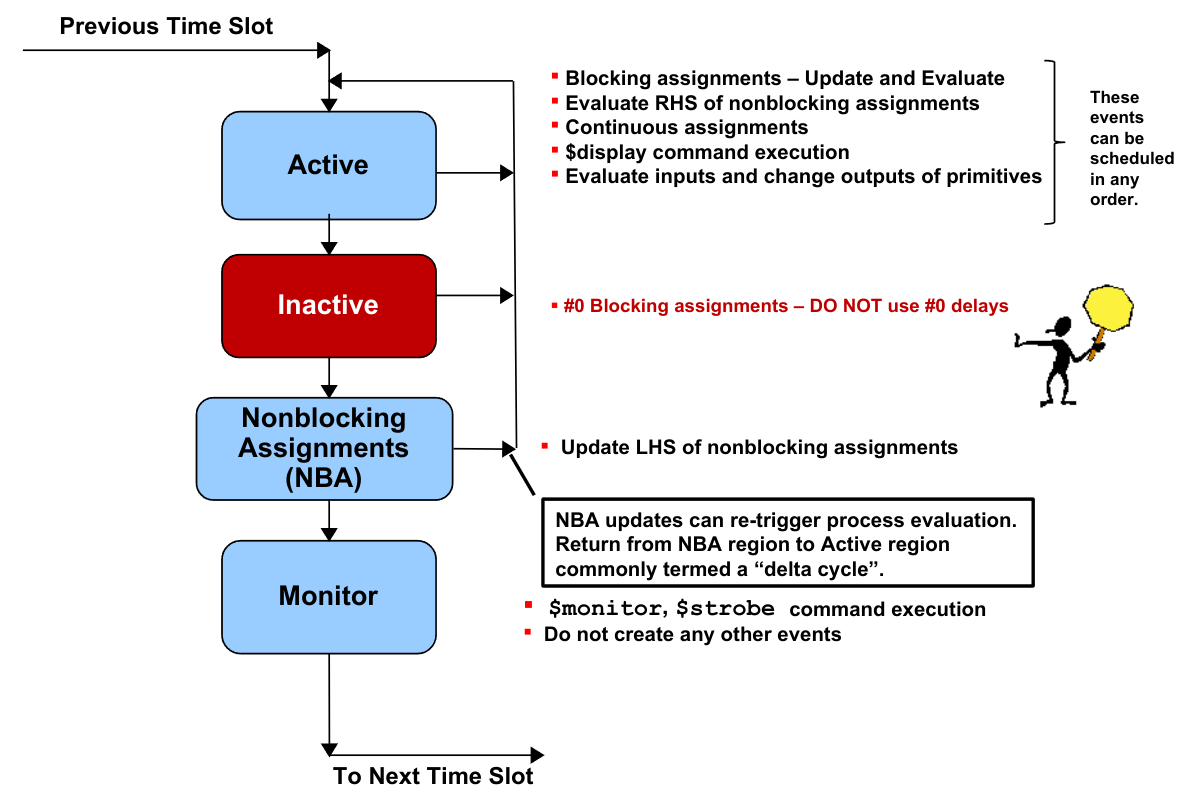
\includegraphics[width=0.95\textwidth]{img/09_event_queue.png}
\end{figure}
\end{frame}
\note{
\scriptsize{
A simulation timeslot is divided into ordered regions to provide a predictable interaction between design constructs.
\newline

The Verilog event schedule has four regions for each simulation time:
\begin{itemize}
\item The Active region is for executing process statements.
\item The Inactive region is for executing process statements postponed with a zero (\#0) procedural delay.
\item The NBA region is for updating non-blocking assignments.
\item The Monitor region is for executing \$monitor and \$strobe and for calling user routines registered for execution during this read-only region. We cannot create additional events during this region
\end{itemize}
The first three of these regions are iterative. They can schedule events that require return to the Active region. When no more events exist for current simulation time, the simulator executes Monitor statements and then advances simulation time to the next time for which events are scheduled. The simulation terminates when no such future events exist.

}
}


%%%%%%%%%%%%%%%%%%%%%%%%%%%%%%%%%%%%%%%%%%%%%%%%%%%%%%%%%%%%
\begin{frame}
\frametitle{Simulation Cycle: 1/6}
\begin{figure}
    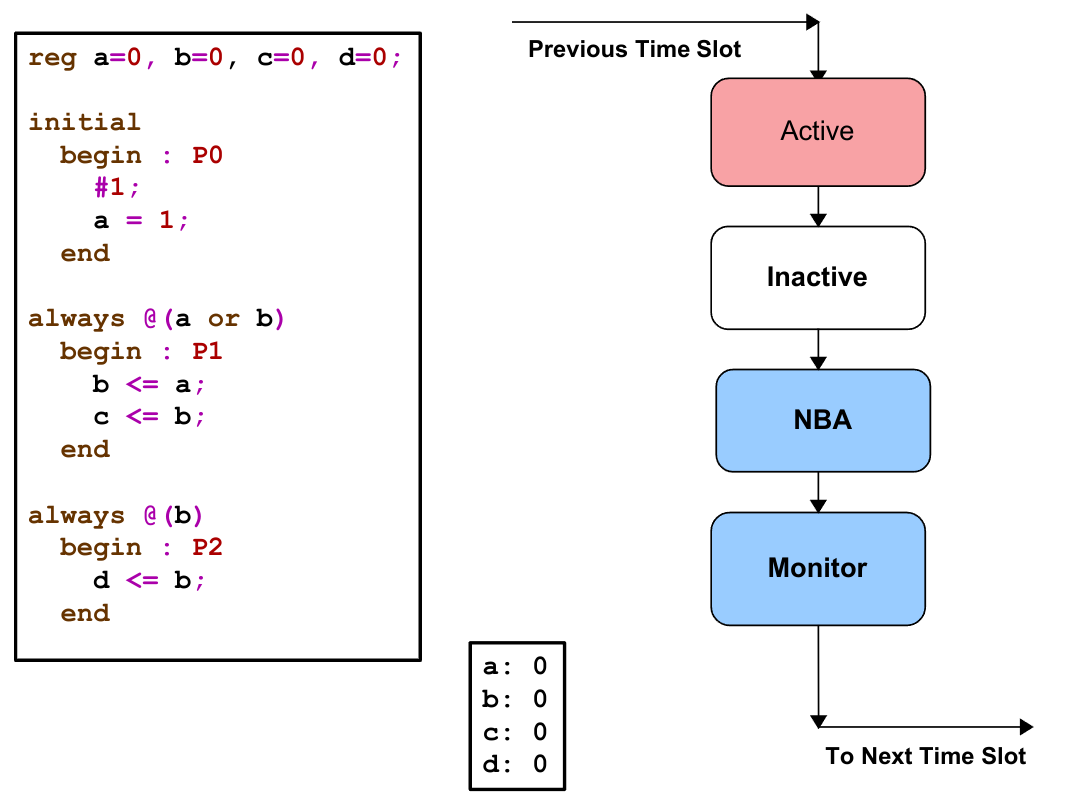
\includegraphics[width=0.95\textwidth]{img/09_cycle_1.png}
\end{figure}
\end{frame}
\note{
\scriptsize{
To demonstrate the behaviour of non-blocking assignments at the simulation cycle, consider a module with three procedures, P1, P1 and P2. 
P1 is an always procedure triggered by an event on a or b. When either event occurs, procedure P1 makes non-blocking assignments to variable \textit{b} and variable \textit{c}, and returns to the top of the loop to again block. P2 also is an always procedure triggered by an event on variable \textit{b}. When the event occurs, procedure P2 makes a non-blocking assignment to variable \textit{d}, and returns to the top of the loop to again block.
When an event occurs on variable \textit{b}, the P1 and P2 processes will resume in either order. This order is predetermined by the simulator and you cannot know or affect it.
\newline

As the simulation starts at time 0, the simulator moves all procedural blocks to the active evaluate events queue, and evaluates them in any order:
\begin{itemize}
\item As the simulator evaluates procedure P0, it immediately encounters a simple delay of \#1, so schedules P0 resumption for the later time.
\item As the simulator evaluates procedures P1 and P2, it immediately encounters event controls, so blocks further execution until one of the associated events occurs.
\end{itemize}

}
}



%%%%%%%%%%%%%%%%%%%%%%%%%%%%%%%%%%%%%%%%%%%%%%%%%%%%%%%%%%%%
\begin{frame}
\frametitle{Simulation Cycle: 2/6}
\begin{figure}
    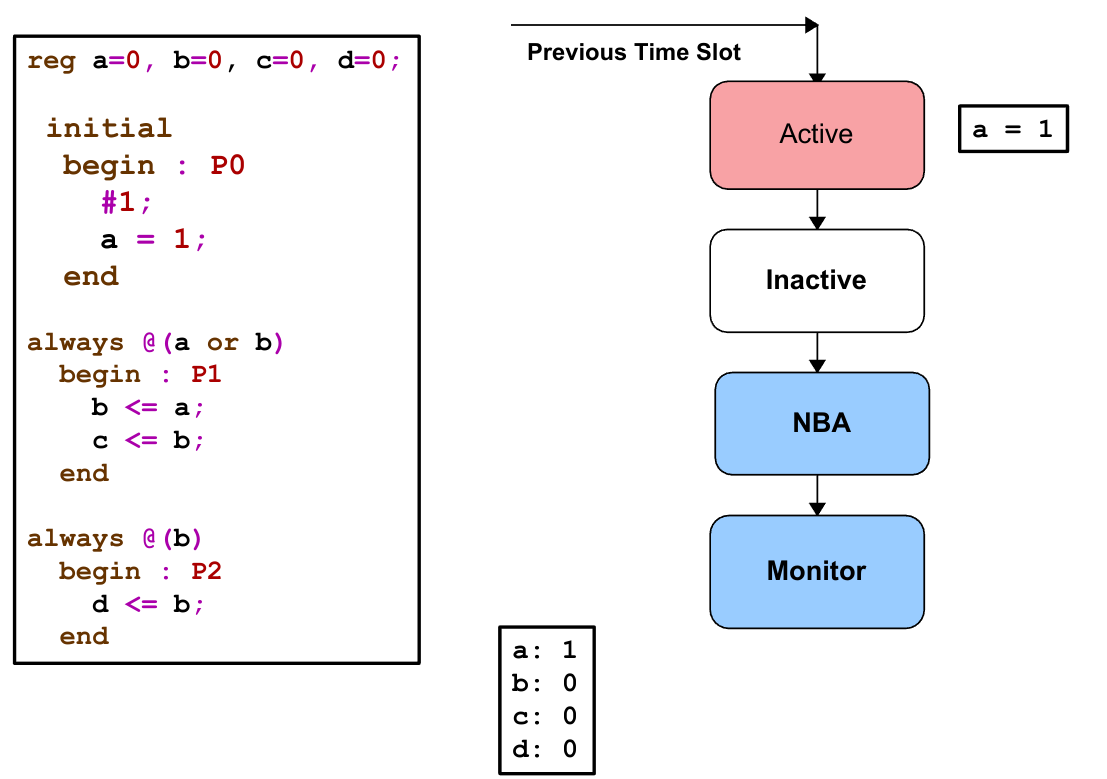
\includegraphics[width=0.95\textwidth]{img/09_cycle_2.png}
\end{figure}
\end{frame}
\note{
\scriptsize{
After exhausting all events at the current time, the simulator jumps to the next event time, and resumes execution of P0.
\newline

Here, the P0 procedure makes an immediate blocking assignment to register \textit{a}, after which P0 completes.
\newline

When the simulator reaches the end of the active region, it checks to see if any procedural blocks have been triggered by the executing blocking assignments. Here a change in value of \textit{a} triggers P1.

}
}


%%%%%%%%%%%%%%%%%%%%%%%%%%%%%%%%%%%%%%%%%%%%%%%%%%%%%%%%%%%%
\begin{frame}
\frametitle{Simulation Cycle: 3/6}
\begin{figure}
    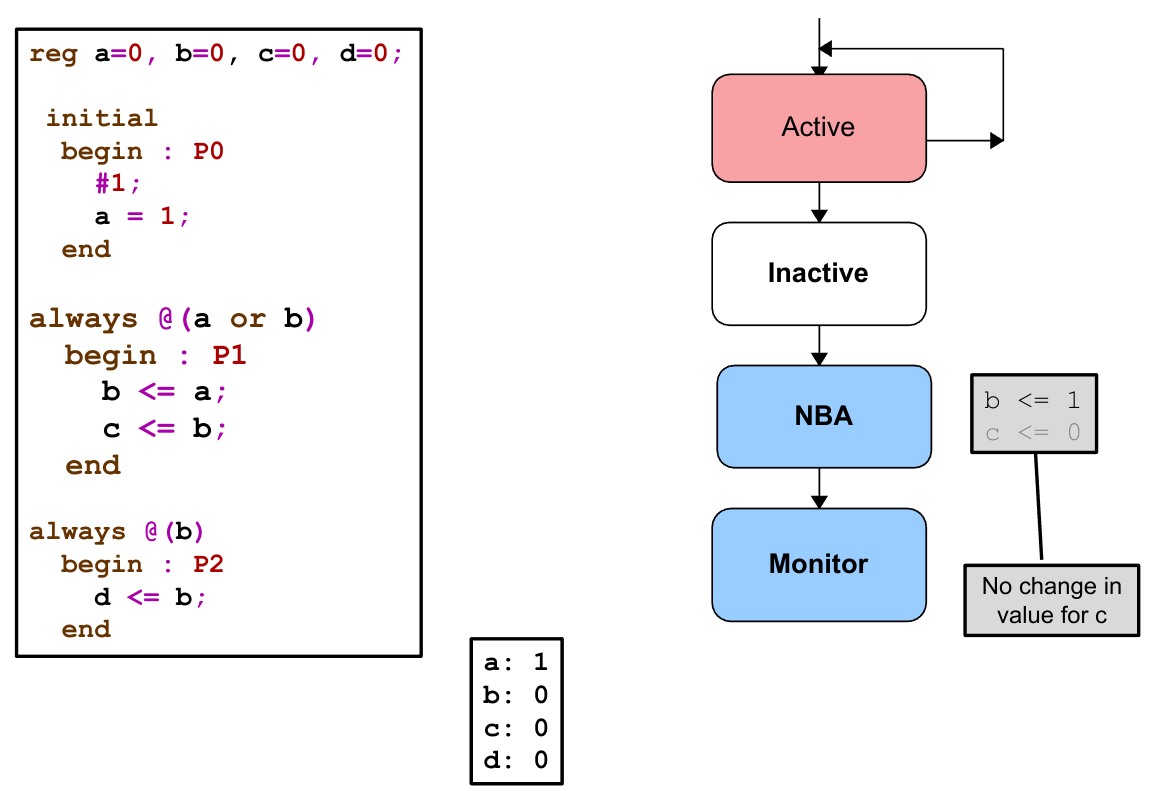
\includegraphics[width=0.95\textwidth]{img/09_cycle_3.png}
\end{figure}
\end{frame}
\note{
\scriptsize{
The simulator re-enters the Active region to execute P1. P1 makes non-blocking assignments to \textit{b} and \textit{c}. These are scheduled for NBA region. Remember non-blocking assignments are evaluated using the current values of variables, therefore \textit{c} is assigned to the current value of \textit{b} which is 0. This is not a new value for \textit{c}, so the assignment can be ignored.

}
}



%%%%%%%%%%%%%%%%%%%%%%%%%%%%%%%%%%%%%%%%%%%%%%%%%%%%%%%%%%%%
\begin{frame}
\frametitle{Simulation Cycle: 4/6}
\begin{figure}
    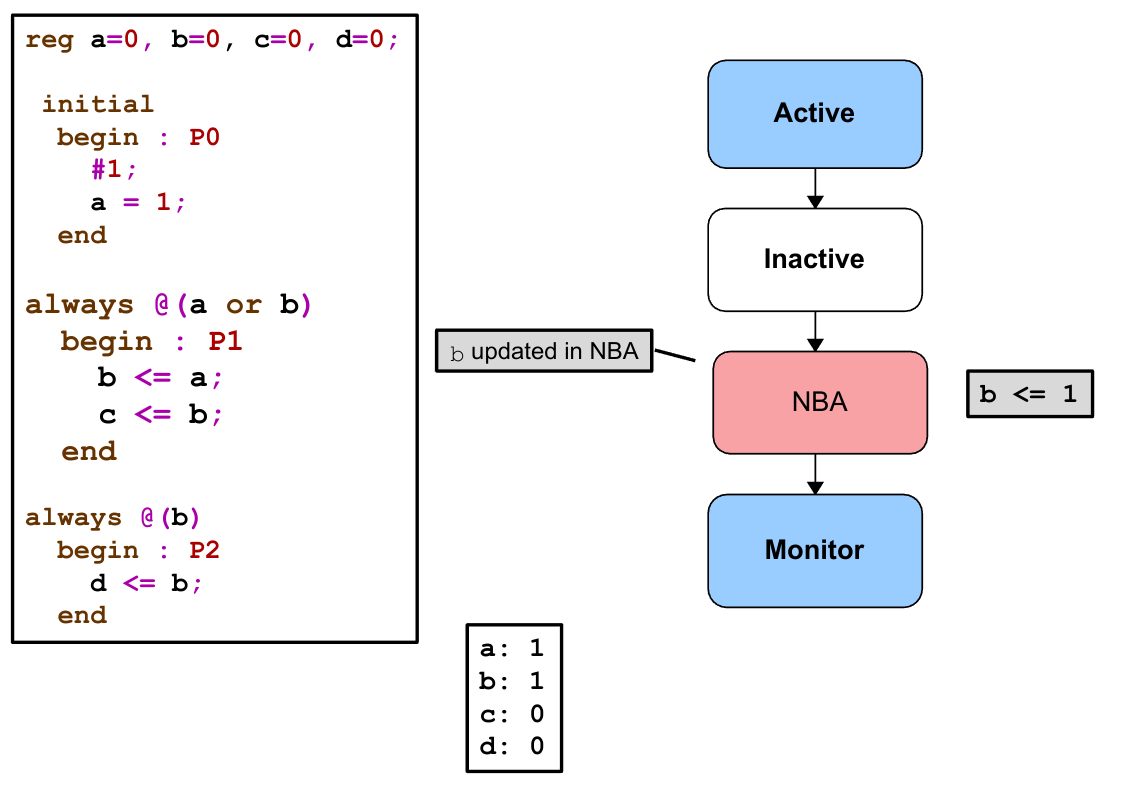
\includegraphics[width=0.95\textwidth]{img/09_cycle_4.png}
\end{figure}
\end{frame}
\note{
\scriptsize{
There are no more procedural blocks triggered by activity in the Active region, therefore the simulator can advance to the NBA region to make the scheduled assignments to \textit{b}.
\newline

When the simulator has completed all the non-blocking assignments in the NBA region, it checks to see if any procedural blocks have been triggered by the assignments. Here a change in the value of \textit{b} triggers P1 and P2.

}
}


%%%%%%%%%%%%%%%%%%%%%%%%%%%%%%%%%%%%%%%%%%%%%%%%%%%%%%%%%%%%
\begin{frame}
\frametitle{Simulation Cycle: 5/6}
\begin{figure}
    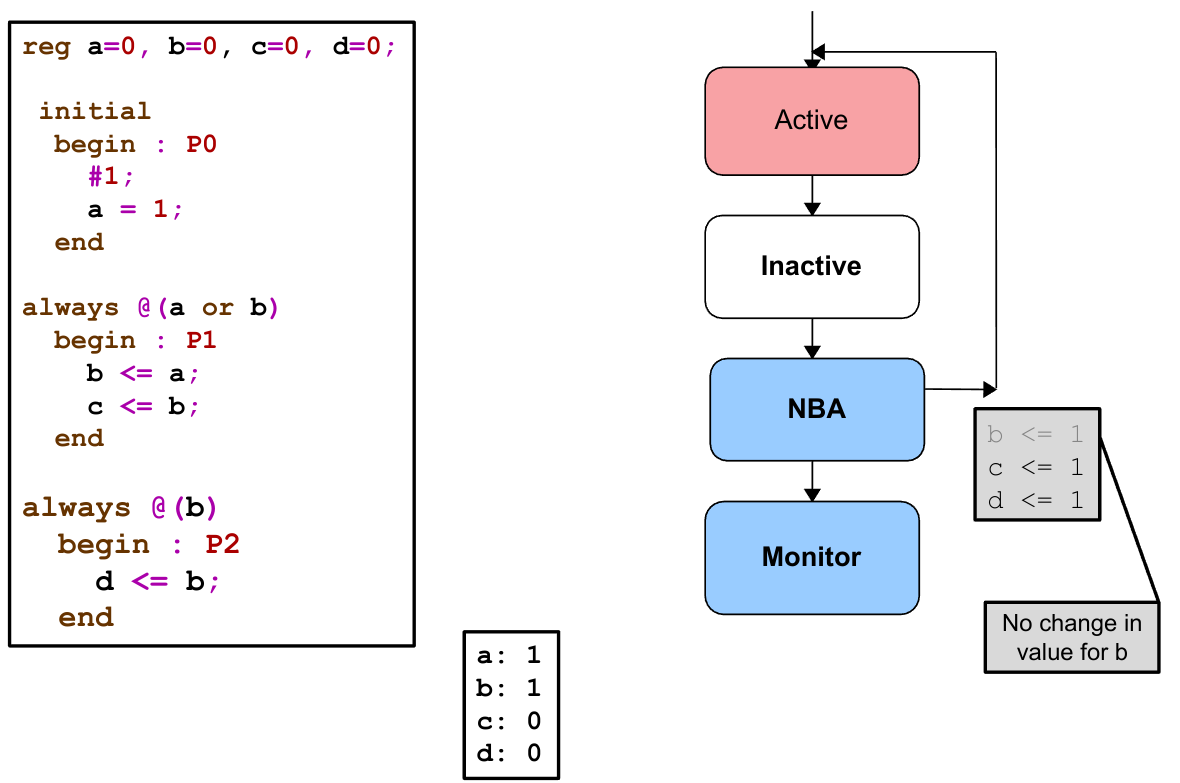
\includegraphics[width=0.95\textwidth]{img/09_cycle_5.png}
\end{figure}
\end{frame}
\note{
\scriptsize{
The simulator re-enters the Active region to execute P1 and P2.
\newline

P1 makes non-blocking assignments to \textit{b} and \textit{c}. These are scheduled for the NBA region. Only \textit{c} receives a new value, therefore the assignment to \textit{b} can be ignored.
\newline

P2 makes the non-blocking assignment to \textit{d}. This is scheduled for the NBA region.
\newline

The execution loop of re-entering the Active region from the NBA region is called a delta cycle. There may be many delta cycles at a given time slot before the simulation reaches a steady state.

}
}


%%%%%%%%%%%%%%%%%%%%%%%%%%%%%%%%%%%%%%%%%%%%%%%%%%%%%%%%%%%%
\begin{frame}
\frametitle{Simulation Cycle: 6/6}
\begin{figure}
    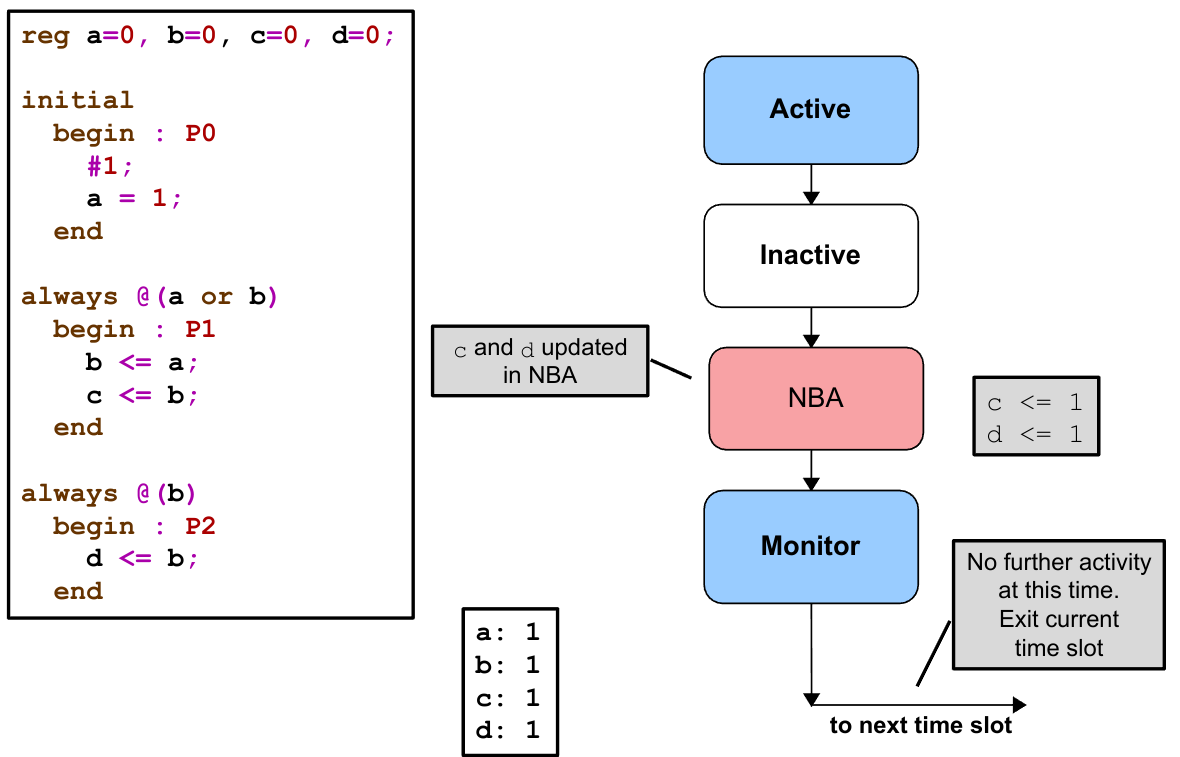
\includegraphics[width=0.95\textwidth]{img/09_cycle_6.png}
\end{figure}
\end{frame}
\note{
\scriptsize{
There are no more procedural blocks triggered by activity in the Active region, therefore the simulator advance to the NBA region to make the scheduled assignments to \textit{c} and \textit{d}.
\newline

When the simulator has completed all the non-blocking assignments in the NBA region, it checks to see if any procedural blocks have been triggered by the assignments. Here there are no triggered blocks, therefore the simulator can exit the current time slot.
\newline

Simulator time will advance to the next nearest event, or if no events are scheduled, the simulator will terminate.

}
}


%%%%%%%%%%%%%%%%%%%%%%%%%%%%%%%%%%%%%%%%%%%%%%%%%%%%%%%%%%%%
\begin{frame}
\frametitle{Simulation Cycle Summary}
\begin{figure}
    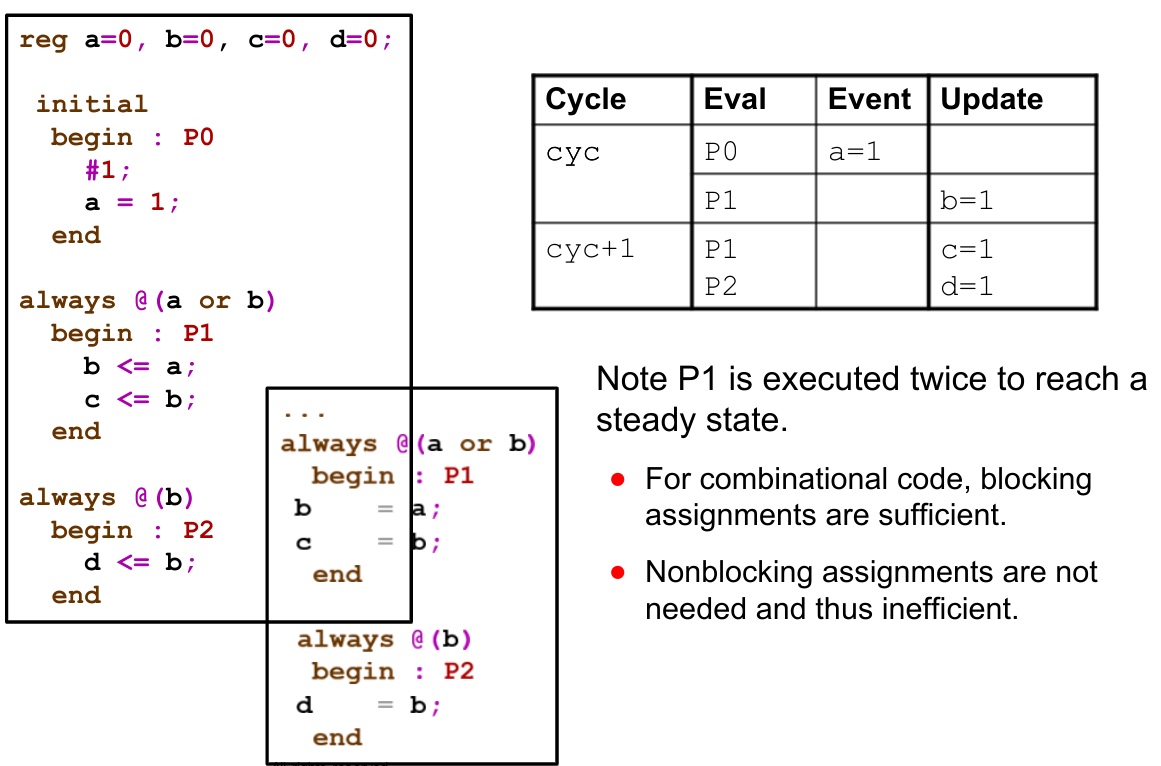
\includegraphics[width=0.95\textwidth]{img/09_cycle_sum.png}
\end{figure}
\end{frame}
\note{
\scriptsize{
Here is a summary of the two delta cycles which propagate the transition of \textit{a} to 1. The first delta cycle evaluates procedure P1, which generates an update event for the assignment to \textit{a}. That update event triggers evaluation of procedure P1, which schedules a non-blocking update to \textit{b} which occurs later in the same delta cycle. The non-blocking update to \textit{b} triggers evaluation of procedures P1 and P2, which occur in the nest delta cycle. These evaluations schedule non-blocking assignments to \textit{c} and \textit{d} that to not affect these procedures.

}
}


%%%%%%%%%%%%%%%%%%%%%%%%%%%%%%%%%%%%%%%%%%%%%%%%%%%%%%%%%%%%
\begin{frame}
\frametitle{Synchronizing Procedures}
\footnotesize{
We can suspend execution of a procedural statement with:
\begin{itemize}
\item The \textcolor{purple}{@} event control (wait for simulation events)
\item \textcolor{purple}{wait} level-sensitive event control (conditionally wait for events)
\item The \textcolor{purple}{\#} delay control (wait for simulation time)
\begin{itemize}
\footnotesize{
	\item Schedules process resumption into the inactive evaluate queue for the current or some future simulation time
}
\end{itemize}
\end{itemize}
\begin{figure}
    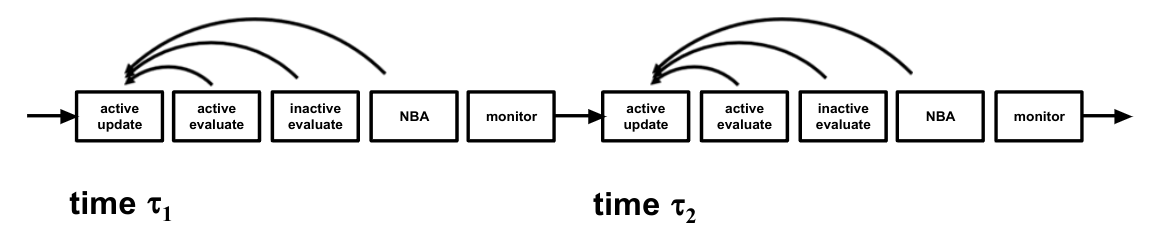
\includegraphics[width=0.95\textwidth]{img/09_sync_proc.png}
\end{figure}

Timing controls are not statements. They apply to the one immediately subsequent statement.
}
\end{frame}
\note{
\scriptsize{
Verilog provides procedural timing controls for \textit{stepping} execution of procedural blocks. Timing controls are not statements. Timing controls apply to the one immediately subsequent statement. In a sequential block, this of course also delays all following statements. Because a timing control is not a statement, it cannot appear at the end of a block unless a statement follows it. Conveniently, that following statement may be a null statement. A null statement is simply a semicolon (;).

}
}


%%%%%%%%%%%%%%%%%%%%%%%%%%%%%%%%%%%%%%%%%%%%%%%%%%%%%%%%%%%%
\begin{frame}[fragile]
\frametitle{Synchronizing Procedures: Event Controls}
\scriptsize{
\begin{multicols}{2}
Use an event control for edge-sensitive timing control behavioural code:
\begin{Verbatim}[commandchars=\\\{\}, tabsize=2]
\textcolor{purple}{		@ event_identifier}
\textcolor{purple}{		@ (event_expression}
\textcolor{purple}{		@*}
\textcolor{purple}{		@ (*)}
\end{Verbatim}
\begin{itemize}
\item An event is any transition of the specified ports, nets or variables
\item Execution resumes when any of the events occur
\item Verilog-2001 added the comma and wild-card operators
\item The wild-card operator adds all signals read within the block and any arguments of functions called from the block
\end{itemize}
\vfill
\columnbreak
\begin{figure}
    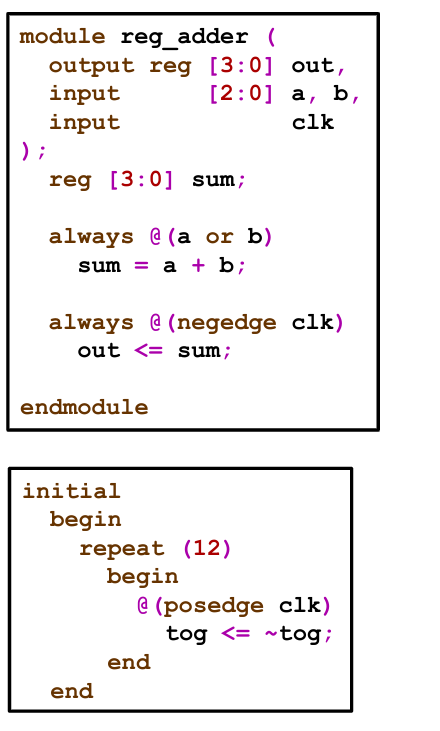
\includegraphics[width=0.4\textwidth]{img/09_sync_proc_event.png}
\end{figure}
\end{multicols}

}
\end{frame}
\note{
\tiny{
Use an event control for edge-sensitive timing control in behavioural code. This is the most commonly used timing control. An event control starts with the \textit{at} (@) character and then follows with either wild-card character, a single event identifier, or a parenthesized event expression. The event expression can be a list of event expressions separated by the \textit{or} keyword or by the comma (,) character. The \textit{or} keyword in an event expression is a separator between event expressions and is not an operator in the usual sense. We can further qualify an expression with the \textit{posedge} or \textit{negedge} keywords.
\newline

This example uses a combinational block to maintain the value of an intermediate sum variable and a sequential block to assign the \textit{sum} value to the output variable upon every negative edge of the clock.
\newline

event\_control ::= 

$|$ \textit{@} event\_identifier

$|$ \textbf{@ (} event\_expression\textbf{)}

$|$ \textbf{@*}

$|$ \textbf{@ (*)}

event\_expression ::=

expression

$|$ hierarchical\_identifier

$|$ \textbf{posedge} expression

$|$ \textbf{negedge} expression

$|$ event\_expression \textbf{or} event\_expression

$|$ event\_expression \textbf{,} event\_expression
\newline

\textbf{Note}: Wild-card event list adds all signals read within the block and any \textbf{arguments} of functions called from the block. If we read a signal in a function via side-effects (i.e., read directly and not passed by the argument list) then that signal is not included in the wild-card event list which is a feature of Verilog 2001.

}
}


%%%%%%%%%%%%%%%%%%%%%%%%%%%%%%%%%%%%%%%%%%%%%%%%%%%%%%%%%%%%
\begin{frame}[fragile]
\frametitle{Synchronizing Procedures: level-Sensitive Event Controls}
\scriptsize{
\begin{multicols}{2}
Use a \textcolor{purple}{wait} statement for level-sensitive timing control in behavioural code:
\begin{Verbatim}[commandchars=\\\{\}, tabsize=2]
\textcolor{purple}{		\textbf{wait (expr)} statement}
\end{Verbatim}

When the statement executes:
\begin{itemize}
\item If the expression is known and true, it does not suspend the process
\item If the expression is unknown or false, it does suspend the process until the expression is known and true
\end{itemize}
\vfill
\columnbreak
\begin{figure}
    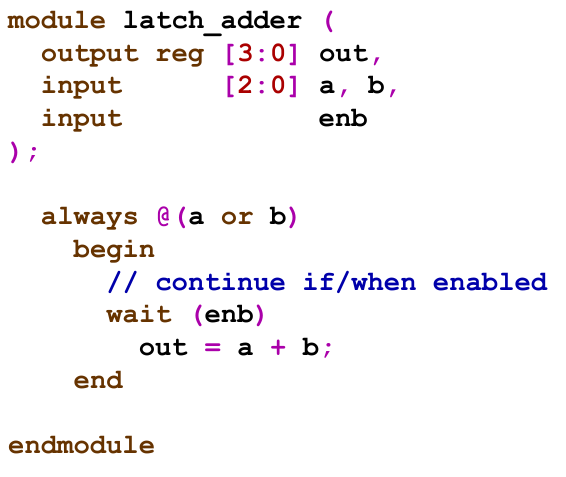
\includegraphics[width=0.45\textwidth]{img/09_sync_proc_level.png}
\end{figure}
\end{multicols}
}
\end{frame}
\note{
\scriptsize{
Use a \textit{wait} statement for level-sensitive timing control in behavioural code, If upon executing the \textit{wait} statement the expression is already true the statement does not block. If upon executing the \textit{wait} statement the expression is not true then the statement does block, and then unblocks if and when the expression becomes true.
\newline

In this example, the procedural block blocks upon every execution until an event occurs on its \textit{a} or \textit{b} inputs. When one of these events occurs, the procedural block tests the state of the enable (\textit{enb}) input, and if the enable input is not 1 then the procedural block again blocks until the enable input becomes 1. While the procedural block is waiting for the enable input to become 1 it misses any further events on the \textit{a} or \textit{b} inputs, as it is not \textit{waiting} for then.
\newline

The wait statement blocks if the expression is not true and then unblocks when the expression becomes true.

}
}


%%%%%%%%%%%%%%%%%%%%%%%%%%%%%%%%%%%%%%%%%%%%%%%%%%%%%%%%%%%%
\begin{frame}[fragile]
\frametitle{Synchronizing Procedures: Delay Control}
\scriptsize{
\begin{multicols}{2}
Use a delay control for a simple time delay:
\begin{Verbatim}[commandchars=\\\{\}, tabsize=2]
\textcolor{purple}{	# delay_value}
\textcolor{purple}{	# ( expr )}
\textcolor{purple}{	# ( expr:expr:expr)}\textcolor{blue}{ // min:typ:max}
\end{Verbatim}
\begin{itemize}
\item For modeling propagation delay
\item For generating a clock
\item For stepping the testbench
\end{itemize}
\vfill
\columnbreak
\begin{figure}
    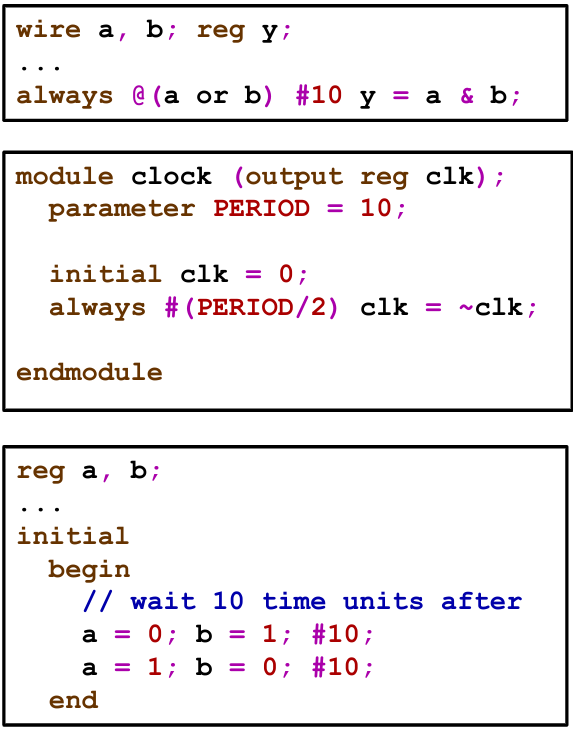
\includegraphics[width=0.45\textwidth]{img/09_sync_proc_delay.png}
\end{figure}
\end{multicols}
}
\end{frame}
\note{
\scriptsize{
Use a delay control for a simple time delay for modeling propagation delay, generating a clock and stepping the testbench. If the delays are constants then we can use module parameters to propagate the constants through the hierarchy.

}
}

%%%%%%%%%%%%%%%%%%%%%%%%%%%%%%%%%%%%%%%%%%%%%%%%%%%%%%%%%%%%
\begin{frame}
\frametitle{Example Timing Controls}
\begin{figure}
    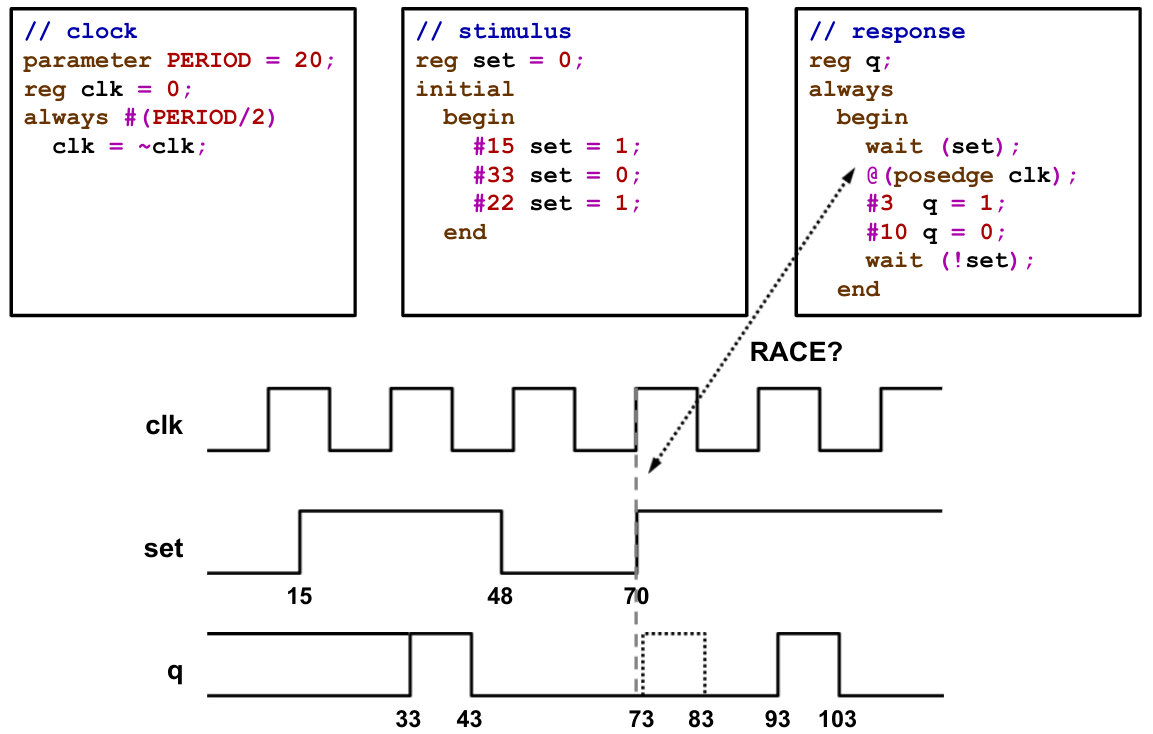
\includegraphics[width=0.95\textwidth]{img/09_timing_control.png}
\end{figure}
\end{frame}
\note{
\tiny{
This example illustrates a collection of timing controls.
\newline

The response procedure does the following:
\begin{enumerate}
\item It waits for "set" to be 1, ignoring the positive clock edge at time 10.
\item After "set" is 1 at time 15, it waits for the positive clock edge.
\item After the positive clock edge at time 30 it waits 3 time units before setting "q" to 1.
\item After setting "q" to 1 at time 33 it waits 10 time units before setting "q" to 0.
\item After setting "q" to 0 at time 43 it waits for "set" to be 0.
\item After "set" is 0 at time 48 it again waits for "set" to be 1.
\item "set" is 1 at time 70, coincident with the positive clock edge. Both assignment statements are on the active evaluate queue. Update to the "set" variable unblocks the response procedure and places it on the active evaluate queue, normally but not necessarily at the end of the queue, so the response procedure normally resumes execution after the positive clock edge has occurred and must wait for the next positive clock edge.
\end{enumerate}
This illustration provides good arguments for synchronizing stimulus to the clock:
\begin{enumerate}
\item The stimulus does not utilize the clock period constant. The stimulus causes greatly different results upon changing the clock period.
\item The stimulus is not synchronized to the clock. If the stimulus is synchronized to the clock,then we know that when the "set" signal transitions, the clock has already occurred and no race condition exist.
\end{enumerate}
}
}

%%%%%%%%%%%%%%%%%%%%%%%%%%%%%%%%%%%%%%%%%%%%%%%%%%%%%%%%%%%%
\begin{frame}[fragile]
\frametitle{Compiler Directive `timescale Preview}
\scriptsize{
\begin{multicols}{2}
The \textcolor{purple}{`timescale} compiler directive specifies the time unit and time precision for all following modules.
\begin{Verbatim}[commandchars=\\\{\}, tabsize=2]
\textcolor{purple}{		`timescale unit/precision}
\end{Verbatim}
\begin{itemize}
\item Can appear only outside module descriptions.
\item Time values in a module are rounded to the precision of that module.
\item The overall simulation time precision is the smallest precision that any module specified.
\end{itemize}
\vfill
\columnbreak
\begin{figure}
    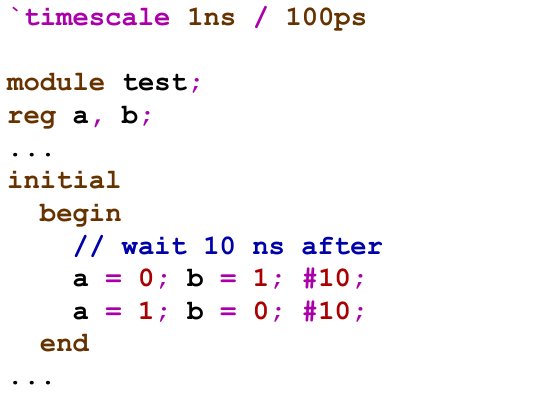
\includegraphics[width=0.45\textwidth]{img/09_timescale.png}
\end{figure}
\end{multicols}
}
\end{frame}
\note{
\tiny{
The \textit{`timescale} directive specifies the time unit and time precision for subsequent module declarations. Any expression used in a context to mean simulation time will assume the time unit of the current module and be rounded to the time precision of the current module. System tasks that display simulation time will scale the display to the time unit of the current module.
\newline

As the standard does not prescribe a default time scale, for interoperability, either all modules must be subject to a time scale or no module can be subject to a time scale. To ensure that all modules are subject to a time scale, we should get used to specifying a time scale at the top of every file, even if we not use time specifications in the file. To modify a time scale, we need to edit the file and recompile that file and all other files that utilized that directive. No method exists to modify a time scale during simulation.
\newline

`timescale time\_unit/time\_precision

\begin{itemize}
\item The \textit{time\_unit} argument specifies the assumed time for time values
\item The \textit{time\_precision} argument cannot be larger than the \textit{time\_unit} argument.
\item Time values are rounded to meed the current precision specification.
\item The overall simulation time precision is the smallest specified time precision.
\item The integer part of the arguments specify a magnitude (1, 100, 1000) and the character string argument suffix is the unit (s, ms, us, ns, ps, fs).
\end{itemize}

}
}

%%%%%%%%%%%%%%%%%%%%%%%%%%%%%%%%%%%%%%%%%%%%%%%%%%%%%%%%%%%%
\begin{frame}
\frametitle{Module Summary}
Now we can produce higher quality code less affected by non-determinism and race conditions.
\newline

This module described:
\begin{itemize}
\item Procedural \textbf{initial} and \textbf{always} blocks
\item Blocking \textbf{=} procedural assignment
\item Non-blocking \textbf{\textless =} procedural assignment
\item The simulation cycle (delta cycles)
\item Timing control
\begin{itemize}
	\item The \textbf{@} event control
	\item The \textbf{wait} level-sensitive event control
	\item The \textbf{\#} delay control
\end{itemize}
\end{itemize}
\end{frame}
\note{
\scriptsize{
Our objective is to produce higher quality code less subject to indeterminacy and race conditions. To do that, we need to understand something about how the simulator executes processes and their statements.

}
}

%%%%%%%%%%%%%%%%%%%%%%%%%%%%%%%%%%%%%%%%%%%%%%%%%%%%%%%%%%%%
\begin{frame}
\frametitle{Module Review}
\begin{enumerate}
\item When does the variable vale change when using a:
\begin{itemize}
	\item blocking assignments
	\item non-blocking assignments
\end{itemize}
\item What are the three Verilog Timing controls?
\item What Verilog construct do you use in a procedure to advance simulation time?
\item Where can you place the \textbf{`timescale} compiler directive?
\end{enumerate}
\end{frame}
\note{
\tiny{
\begin{enumerate}
\item When does the variable vale change when using a:
\begin{itemize}
	\tiny{
	\item blocking assignments
	\begin{itemize}
	\tiny{
		\item A blocking assignment blocks execution of subsequent statements of the procedure until the assignment completes, which is by default immediately.
	}
	\end{itemize}
	\item non-blocking assignments
	\begin{itemize}
	\tiny{
		\item A non-blocking assignment schedules assignment completion for the "update" phase of delta cycle, by default the current cycle.
	}
	\end{itemize}
	}
\end{itemize}
\item What are the three Verilog Timing controls?
\begin{itemize}
	\tiny{
		\item The \textbf{@} event control, the \textbf{wait} level-sensitive event control, the \textbf{\#} delay control.
	}
\end{itemize}
\item What Verilog construct do you use in a procedure to advance simulation time?
\begin{itemize}
	\tiny{
		\item The \textbf{\#} delay control suspends the procedure for a specified simulation time.
	}
\end{itemize}
\item Where can you place the \textbf{`timescale} compiler directive?
\begin{itemize}
	\tiny{
		\item In the source code outside any module definition. The Verilog standard implies but not does explicitly specify this by saying it applies to "modules that follow" and always showing it outside example modules.
	}
\end{itemize}
\end{enumerate}
}
}

%%%%%%%%%%%%%%%%%%%%%%%%%%%%%%%%%%%%%%%%%%%%%%%%%%%%%%%%%%%%
\begin{frame}
\frametitle{Lab}
Lab 10-1 Modeling a Generic Counter
\begin{itemize}
\item Use blocking and non-blocking assignments while describing a counter.
\end{itemize}
\begin{figure}
    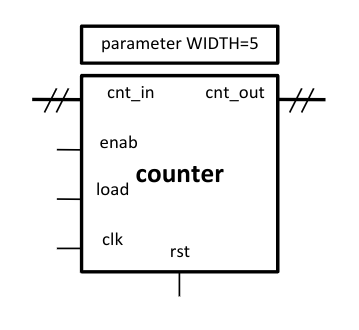
\includegraphics[width=0.45\textwidth]{img/09_lab.png}
\end{figure}
\end{frame}


%%%%%%%%%%%%%%%%%%%%%%%%%%%%%%%%%%%%%%%%%%%%%%%%%%%%%%%%%%%%
\begin{frame}
\frametitle{Test Your Understanding - 1}
In which order does the simulator processes these regions of the stratifies event queue?
\begin{itemize}
\item[$\square$] inactive, active, monitor, NBA
\item[$\square$] monitor, inactive, active, NBA
\item[$\square$] inactive, active, NBA, monitor
\item[$\square$] active, inactive, monitor, NBA
\item[$\square$] active, inactive, NBA, monitor
\end{itemize}
\end{frame}
\note{
In which order does the simulator processes these regions of the stratifies event queue?
\begin{itemize}
\item[$\square$] inactive, active, monitor, NBA
\item[$\square$] monitor, inactive, active, NBA
\item[$\square$] inactive, active, NBA, monitor
\item[$\square$] active, inactive, monitor, NBA
\item[$\boxtimes$] active, inactive, NBA, monitor
\end{itemize}
}


%%%%%%%%%%%%%%%%%%%%%%%%%%%%%%%%%%%%%%%%%%%%%%%%%%%%%%%%%%%%
\begin{frame}
\frametitle{Test Your Understanding - 2}
For which procedural assignment does the simulator update "lvalue" in the same simulation cycle that it evaluates the "rvalue" if a "simulation cycle" is the processing of currently active events as defined for the stratified event queue?
\begin{itemize}
\item[$\square$] \#0 lvalue = rvalue;
\item[$\square$] \#0 lvalue \textless = rvalue;
\item[$\square$] lvalue \textless = \#0 rvalue;
\item[$\square$] lvalue = \#0 rvalue;
\end{itemize}
\end{frame}
\note{
For which procedural assignment does the simulator update "lvalue" in the same simulation cycle that it evaluates the "rvalue" if a "simulation cycle" is the processing of currently active events as defined for the stratified event queue?
\begin{itemize}
\item[$\boxtimes$] \#0 lvalue = rvalue;
\item[$\square$] \#0 lvalue \textless = rvalue;
\item[$\square$] lvalue \textless = \#0 rvalue;
\item[$\square$] lvalue = \#0 rvalue;
\end{itemize}

}

%%%%%%%%%%%%%%%%%%%%%%%%%%%%%%%%%%%%%%%%%%%%%%%%%%%%%%%%%%%%
\begin{frame}
\frametitle{Test Your Understanding - 3}
Which one or more of these are syntactically valid procedures?
\begin{itemize}
\item[$\square$] always begin c = $\sim$ c; \#1 end
\item[$\square$] always begin \#1 c = $\sim$ c; end
\item[$\square$] always begin \#1; c = $\sim$ c; end
\item[$\square$] always begin c = $\sim$ c; \#1; end
\end{itemize}
\end{frame}
\note{
Which one or more of these are syntactically valid procedures?
\begin{itemize}
\item[$\square$] always begin c = $\sim$ c; \#1 end
\item[$\boxtimes$] always begin \#1 c = $\sim$ c; end
\item[$\boxtimes$] always begin \#1; c = $\sim$ c; end
\item[$\boxtimes$] always begin c = $\sim$ c; \#1; end
\end{itemize}

}


%%%%%%%%%%%%%%%%%%%%%%%%%%%%%%%%%%%%%%%%%%%%%%%%%%%%%%%%%%%%
\begin{frame}
\frametitle{Test Your Understanding - 4}
You code a wait(1) level-sensitive event control to:
\begin{itemize}
\item[$\square$] wait because its argument is true
\item[$\square$] wait one time unit
\item[$\square$] wait one simulation cycle
\item[$\square$] not wait because its expression is true
\end{itemize}
\end{frame}
\note{
You code a wait(1) level-sensitive event control to:
\begin{itemize}
\item[$\square$] wait because its argument is true
\item[$\square$] wait one time unit
\item[$\square$] wait one simulation cycle
\item[$\boxtimes$] not wait because its expression is true
\end{itemize}

}



\end{document}
